%!mode::"Tex:UTF-8"
\documentclass{ctexart}
\usepackage{fullpage}
\usepackage{parskip}
\usepackage{physics}
\usepackage{amsmath}
\usepackage{amssymb}
\usepackage{xcolor}
%\usepackage[colorlinks,urlcolor=blue]{hyperref}
\usepackage{array}
\usepackage{longtable}
\usepackage{multirow}
\usepackage{comment}
\usepackage{graphicx}
\usepackage{cite}

\title{关于最近做的一些计算}
\author{黄应生}
\date{}

\begin{document}
\maketitle
\tableofcontents

\section{薛定谔方程的数值解}
目前我采用的方法还只是利用Mathematica预置的NDSolve函数求解薛定谔方程,基本步骤是以能量本征值E为参数求解微分方程的数值解,并用FindRoot函数求出满足波函数边值条件的E的值。
\subsection{第一个尝试:一维有限深方势阱}
一维有限深方势阱是我所做的第一个尝试。

方势阱$V(x)$势函数为:
\begin{equation}
V(x)=
\begin{cases}
  V_0, & \;\;\;\abs{x}\leq a \\
  0, &  \;\;\;\abs{x}>a
\end{cases}
\text{\;\;,}\end{equation}
其中$V_0=-3eV$,$a=2\text{\r{A}}$。将之代入一维定态薛定谔方程
\begin{equation}\label{Schrodinger}
  \bqty{-\frac{\hbar^2}{2m}\dv[2]{x}+V(x)}\psi(x)=E\psi(x)
\end{equation}
中,进行求解,可以得到含参数$E$的微分方程如下:
\begin{equation}\label{SquareEq}
  \dv[2]{x}\psi(x)+\alpha\bqty{E-V(x)}\psi(x)=0
\end{equation}
其中$\displaystyle\alpha=\frac{\hbar^2}{2m}$。

要对\eqref{SquareEq}进行求解,可以使用ParameterNDSolve函数或者NDSolve函数(采取边界条件为$\psi(x_1)=\psi_0$,$\displaystyle\dv{x}\psi(x_1)=\sqrt{-\alpha\bqty{E-V(x_1)}}$(根据Sturm引理),$\psi_0=1.0\times10^{-3}$)。前者只需规定参数为$E$后直接进行求解,后者则需要设一个以$E$为变量的函数$f(e)$,即为解出的带参数$E$的波函数在边界如$x_2=a$处的值,最后只需令ParameterNDSolve函数解出的含参数函数在如$x_2=a$这样的边界上的值或者是$f(e)$满足题设的边界条件,利用FindRoot函数即可解出最终的能量本征值,两种方法本质上区别不大。在这里以$x_2=a$处为例,考虑$x_2$处需满足的边界条件:偶宇称情况下,由对称性及之前所设初值条件,波函数值可设为$\psi_0$,$\psi_0=1.0\times10^{-3}$;奇宇称情况下,波函数值可设为$-\psi_0$。由此解出两个能量本征值(在后面的部分均默认能量单位为$eV$):
\[
\left\{
\begin{array}{l}
  E_1 = -2.07927\;\; eV\\
  E_2 = -0.0930281\;\;eV
\end{array}
\right.
\]
\subsection{氢原子库伦势}
与上面的讨论类似,对于氢原子的库伦势,可以把三维定态薛定谔方程进行分离变量,得到径向方程
\begin{equation}\label{radiusEq}
  -\frac{\hbar^2}{2m}\dv[2]{u}{r}+\bqty{V(r)+\frac{\hbar^2}{2m}\frac{l(l+1)}{r^2}}u=Eu
\end{equation}
其中$u(r)\equiv rR(r)$。相似地,利用$u(r)$在无穷远处函数值趋于0,导数是负的且同样趋于0,在原点处函数值趋于0的性质,可以写出边界条件
\begin{equation*}
\begin{cases}
u(r_1)&=u0\\
u'(r_1)&=-\sqrt{-\alpha\bqty{E-V(r_1)}}
\end{cases}
,
\end{equation*}
并用FindRoot函数类似进行求解。

计算出的能量本征值($l=0$)如表1,
\begin{table}[!htdp]
  \centering
  \begin{tabular}{|c|c|c|c|c|c|c|}
    \hline
    % after \\: \hline or \cline{col1-col2} \cline{col3-col4} ...
    能级 & 1 & 2 & 3 & 4 & 5 & 6 \\
    \hline
    计算值 & -13.6182 & -3.40456 & -1.51314 & -0.851141 & -0.544731 & -0.378285\\
    \hline
    理论值 & -13.6057 & -3.4014 & -1.5117 & -0.8503 & -0.5442 & -0.3779 \\
    \hline
  \end{tabular}
  \caption{氢原子能级}\label{}
\end{table}
从计算值和理论值的对比可以看出仍然存在一定误差,但是总体来说比较接近。误差的存在主要是因为所引用的Schrodinger Constant不够精确,在加大其精度后计算结果的精度得到了很大改善。

\subsection{Short-Range Potential}
仍然类似之前的解法,将氢原子的库伦势改写为
\begin{equation}\label{Vs}
  V=-\frac{e^2}{4\pi \epsilon_0 r}+V_s(r)
\end{equation}
代入径向方程\eqref{radiusEq}中,即可按微分方程的初值问题求解。
\subsubsection{势$V_s$为$\displaystyle\frac{0.1}{r^2}$}
首先设
\begin{equation}
V_s=\frac{0.1}{r^2},
\end{equation}
系数设为0.1是出于能够利用微扰论验证的目的。
类似求解,得到能量本征值。又知若将$\displaystyle V_s=\frac{0.1}{r^2}$看作微扰,则能量的一级微扰(根据F-H定理)为
\begin{eqnarray*}
% \nonumber % Remove numbering (before each equation)
\ev{V_s}{\psi_n^{(0)}} &=& \mel{nlm}{\frac{0.1}{r^2}}{nlm} \\
   &=& \frac{0.2}{(2l+1)a^2n^3}
\end{eqnarray*}\label{}
其中$a$为玻尔半径,$n$为氢原子能级。

最终解出计算值与微扰值($l=0$)见表2:
\begin{table}[!htbp]
  \centering
  \begin{tabular}{|c|c|c|c|c|c|}
    \hline
    % after \\: \hline or \cline{col1-col2} \cline{col3-col4} ...
    能级 & 1 & 2 & 3 & 4 & 5 \\
    \hline
    计算值 & -12.9465 & -3.34907 & -1.48763 & -0.840345 & -0.539192 \\
    \hline
    微扰值 & -12.8853 & -3.31066 & -1.48464 & -0.838833 & -0.538282 \\
    \hline
    相对误差 & 0.472517\% & 1.1469\% & 0.200812\% & 0.1799\% & 0.168726\% \\
    \hline
  \end{tabular}
  \caption{$\displaystyle V_s=\frac{0.1}{r^2}$下的能级}\label{}
\end{table}\\
两组数据的相关性达到$0.999998$。虽然仍存在一定误差,但用作验证的仅是一级微扰,本身不够精确,可以认为计算值有一定参考价值。
\subsubsection{势$V_s$为$\displaystyle\frac{0.1}{r^3}$}
同上,若设
\begin{equation}\label{Vs2}
  V_s=\frac{0.1}{r^3},
\end{equation}
将$V_s$看作微扰,由Kramers关系($\displaystyle\frac{s+1}{n^2}\ev{r^s}-(2s+1)a\ev{r^{s-1}}+\frac{s}{4}\bqty{(2l+1)^2-s^2}a^2\ev{r^{s-2}}=0$) 及之前所得出的$\ev{V_s}$,有
\begin{eqnarray*}
% \nonumber % Remove numbering (before each equation)
 \ev{V_s}{\psi_n^{(0)}} &=& \mel{nlm}{\frac{0.1}{r^3}}{nlm} \\
   &=& \frac{0.1}{l(l+1)a}\ev{\frac{1}{r^2}}_{nlm}  \\
   &=& \frac{0.2}{l(l+1)(2l+1)a^3n^3}
\end{eqnarray*}
由于$l=0$时一级微扰趋于无穷,故计算$l=1$时的能量。

最终得到结果如表3:
\begin{table}[!htbp]
  \centering
  \begin{tabular}{|c|c|c|c|c|c|c|c|}
    \hline
    % after \\: \hline or \cline{col1-col2} \cline{col3-col4} ...
    能级 & 1 & 2 & 3 & 4 & 5 & 6 & 7 \\
    \hline
    计算值 &  & -3.37725 & -1.50504 & -0.847725 & -0.542981 & -0.377272 & -0.277286  \\
    \hline
    微扰值 & -13.3748 & -3.37185 & -1.50277 & -0.846482 & -0.542199 & -0.376735 & -0.276895 \\
    \hline
    相对误差 &  & 0.159701\% & 0.151035\% & 0.14667\% & 0.144081\% & 0.142375\% & 0.14117\% \\
    \hline
  \end{tabular}
  \caption{$\displaystyle V_s=\frac{1}{r^3}$下的能级}\label{}
\end{table}\\
两组数据相关度为$0.9999999994$。基态能量计算时由于$f(e)$在$e$接近-6时就开始上扬,从函数图像上看在-13处并无交点,没有计算出结果。
\section{关于Lepage文的数据计算}
根据所给的三组数据,我首先对其进行了拟合,画出Lepage文中TrueV与$a^2$、$a^4$的有效势的对照图,然后根据拟合得到的TrueV势函数求解薛定谔方程尝试得到Lepage所给出的几个S波能量本征值。关于相移,因为能量的计算还有一些问题没有解决,暂时没有着手计算。
\subsection{对三组数据的拟合}
已知有效势的形式:
\begin{eqnarray*}
% \nonumber % Remove numbering (before each equation)
  V_{eff}(\vb{r}) &=& -\frac{\alpha}{r}\;erf\pqty{\frac{r}{\sqrt{2}a}} \\
   &\phantom{=}& +c\; a^2\;\delta_a^3(\vb{r}) \\
   &\phantom{=}& +d_1\;a^4\;\laplacian{\delta_a^3(\vb{r})}+d_2\;a^4\;\div{\delta_a^3(\vb{r})}\grad \\
   &\phantom{=}& +\dots \\
   &\phantom{=}& +g\;a^{n+2}\;\nabla^n\delta_a^3(\vb{r}) \\
   &\phantom{=}& \dots\;\text{,}
\end{eqnarray*}
其中smeared delta functon定义为$\displaystyle\delta_a^3(\vb{r})=\frac{e^{-\frac{r^2}{2a^2}}}{(2\pi)^{\frac{3}{2}}\;a^3}$。

在精确到$a^2$的情况下,
\begin{equation}
  V_{eff}^{(a^2)}=-\frac{\alpha}{r}\;erf\pqty{\frac{r}{\sqrt{2}a}}+c\; a^2\;\delta_a^3(\vb{r}),
\end{equation}
精确到$a^4$的情况下,
\begin{equation}
  V_{eff}^{(a^4)}=-\frac{\alpha}{r}\;erf\pqty{\frac{r}{\sqrt{2}a}}+c\; a^2\;\delta_a^3(\vb{r})+d_1\;a^4\;\laplacian{\delta_a^3(\vb{r})}+d_2\;a^4\;\div{\delta_a^3(\vb{r})}\grad,
\end{equation}
将之分别作为model代入FindFit函数中求拟合参数,由Lepage给出的条件$a=1$得到最终结果:
\begin{eqnarray}
% \nonumber % Remove numbering (before each equation)
  V_{eff}^{(a^2)} &=& -2.74316\;e^{-\frac{r^2}{2}}-\frac{erf\pqty{\frac{r}{\sqrt{2}}}}{r} \\
  V_{eff}^{(a^4)} &=&  -2.55773\;e^{-\frac{r^2}{2}}+2.36456\pqty{-\frac{3\;e^{-\frac{r^2}{2}}}{2\sqrt{2}\;\pi^{\frac{3}{2}}}+\frac{e^{-\frac{r^2}{2}}\;r^2}{2\sqrt{2}\;\pi^{\frac{3}{2}}}}-\frac{erf\pqty{\frac{r}{\sqrt{2}}}}{r}
\end{eqnarray}
如图1所示。TrueV的曲线拟合因为没有模型,留待下一节解决。
\newpage
\begin{figure}[!htp]
  \centering
  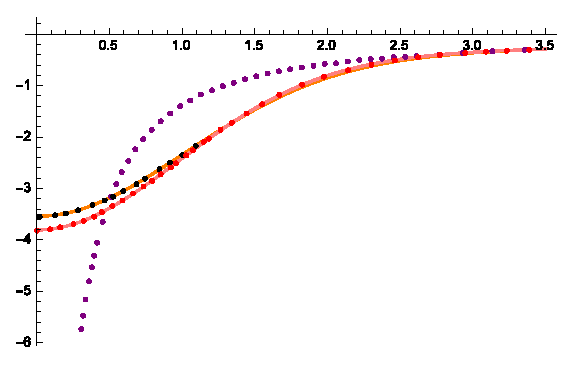
\includegraphics[width=4.50in]{Test_Veff_Three_DiracDelta&SmearedDiracDelta.eps}
  \caption{TrueV、$V_{eff}^{(a^2)}$、$V_{eff}^{(a^4)}$(原始数据点按顺序分别为紫、黑、红,后两者的拟合曲线分别为橙、粉)}
\end{figure}

\subsection{重现Lepage文中的S波能量本征态}
\subsubsection{拟合TrueV}
Lepage文中并没有给出TrueV的具体解析形式。所以我使用Fit函数、FindFit函数进行其拟合函数的试探。最终发现,具备
$$
V(r)=-\frac{a}{r^b}+c\;\frac{e^{-dr}}{r}
$$
形式的拟合函数表现最好,和原始数据的差别最小。由于Lepage原文中是在一个库伦势的基础上建立的,可以作出假设$a=1$且$b=1$。最终拟合结果(对不同的model)为以下三个函数:
\begin{eqnarray}
% \nonumber % Remove numbering (before each equation)
  V_1(r) &=& -\frac{1.09835e^{-1.06921r}}{r}-\frac{1.00409}{r^{0.976102}} \\
  V_2(r) &=& -\frac{1}{r}-\frac{1.04152e^{-0.9991r}}{r} \\
  V_3(r) &=& -\frac{1.38622}{r^{1.21524}}
\end{eqnarray}
$V_2(r)$是在假设$a=1$且$b=1$下拟合出的,$V_3(r)$是以$\displaystyle-\frac{a}{r^b}$为model拟合出的。

我同时还对三个函数和原始的TrueV数据在各点上进行了对比,其函数值与原始数据的平方差(为了易于观察)如图2,可以看出其中$V_1$表现与$V_2$相差无几,但是考虑到库伦势的基础,故并不采用$V_1$。$V_3(r)$在前几个点由于差距较大,超出了图的范围,并未画出。
\clearpage
\begin{figure}[!htbp]
  \centering
  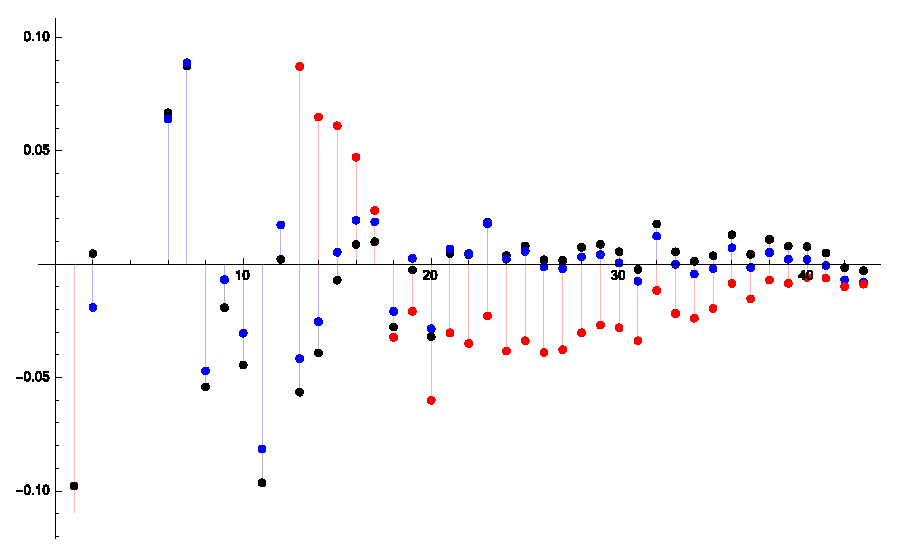
\includegraphics[width=4.5in]{Test_ReconstructLepage.eps}
  \caption{三个函数在原始数据的各点上的对比(函数值平方差,按顺序分别为蓝、黑、红)}\label{TrueV}
\end{figure}

\subsubsection{拟合的TrueV函数为$\displaystyle-\frac{1.38622}{r^{1.21524}}$}
采用$V_3(r)$为TrueV的函数,类似之前的讨论求解。结果如表4。
\begin{table}[!htbp]
  \centering
  \begin{tabular}{|cccccc|}
    \hline
    % after \\: \hline or \cline{col1-col2} \cline{col3-col4} ...
    能级 & 能量计算值 & Lepage能量值 & 能级 & 能量计算值 & Lepage能量值 \\
    \hline
    1S & 1.31401 & 1.28711542 & 6S & 0.0168508 & 0.0155492598 \\
    2S & 0.213295 & 0.183325753  & \dots &   & \\
    3S & 0.0749002 & 0.0703755485 & 10S & 0.00536301 & 0.00534541931 \\
    4S & 0.0387671 & 0.0371495726 & 20S & 0.00126957 & 0.00129205010 \\
    5S & 0.02289 & 0.0229268241  &  &  &  \\
    \hline
  \end{tabular}
  \caption{$V_3\;\;$S波能量对比}
\end{table}
\subsubsection{拟合的TrueV函数为$\displaystyle-\frac{1}{r}-\frac{1.04152e^{-0.9991r}}{r}$}
采用$V_2(r)$为TrueV的函数,类似之前的讨论求解。结果如表5。可以看出总体误差在$1\%$左右,并且能级越高,误差越小,基态的误差最大。除了计算过程中可能的问题外,这也可能是由于$V_2(r)$与Lepage实际使用的势函数仍有不同,且在$r$较小时差别较大的原因。
\clearpage
\begin{table}[!htbp]
  \centering
  \begin{tabular}{|cccccccc|}
    \hline
    % after \\: \hline or \cline{col1-col2} \cline{col3-col4} ...
    能级 & 能量计算值 & Lepage能量值 & 相对误差 & 能级 & 能量计算值 & Lepage能量值 & 相对误差 \\
    \hline
    1S & 1.33732 & 1.28711542 & 3.90057\% & 6S & 0.0156184 & 0.0155492598 & 0.444587\% \\
    2S & 0.186434 & 0.183325753 & 1.69544\% & \dots &   &  & \\
    3S & 0.0710575 & 0.0703755485 & 0.968963\% & 10S & 0.00535929 & 0.00534541931 & 0.259539\% \\
    4S & 0.0374072 & 0.0371495726 & 0.693401\% & 20S & 0.0012937 & 0.00129205010 &0.127336\%\\
    5S & 0.023051 & 0.0229268241 & 0.541494\% &  &  & & \\
    \hline
  \end{tabular}
  \caption{$V_2\;\;$S波能量对比}
\end{table}
\section{目前存在的一些问题}
目前对于数值计算,我的程序在精度的控制上还有很大不足,另外对于高能级的计算仍然误差很大,目前的方法也很不方便,必须要一个能级一个能级地找,也容易出错;同时比较奇怪的一点是基态能量的误差一般偏大,能级变大之后误差会急剧下降。当然我也会继续尝试将微分方程离散后求本征值的方法。
\begin{thebibliography}{1}

\bibitem{dong1}
董键. Mathematica与大学物理计算 第2版[M]. 清华大学出版社, 2013.

\bibitem{G2}
Griffiths, David Jeffery. Introduction to quantum mechanics. Pearson Education India, 2013.

\bibitem{3}
徐安农. 科学计算引论: 基于 Mathematica 的数值分析[M]. 机械工业出版社, 2010.

\bibitem{4}
张晓丹. 应用计算方法教程[M]. 机械工业出版社, 2008.

\bibitem{5}
Lepage P. How to Renormalize the Schrodinger Equation[J]. Nuclear Theory, 1997.

\end{thebibliography}
\end{document} 